\chapter{Experiments and Results}

\section{Data}
The experiments use the two datasets supported by the current codebase:
MNIST and CIFAR-10. Both datasets are stored under the project-local
\path{data/} directory and are loaded through the PyTorch \texttt{torchvision}
dataset interfaces with \texttt{download=True}. No physical wireless-channel
dataset is required, because the channel perturbation is generated
synthetically by the OTA aggregation oracle.

MNIST is used as a lightweight sanity benchmark. It contains 60,000 training
images and 10,000 test images of handwritten digits. The raw files are stored
under \path{data/MNIST/raw/}. Images are converted to tensors and normalized
with mean 0.1307 and standard deviation 0.3081.

CIFAR-10 is used as the main image-classification benchmark. It contains
50,000 training images and 10,000 test images across 10 object classes. The
raw batch files \texttt{data\_batch\_1} through \texttt{data\_batch\_5},
\texttt{test\_batch}, and \texttt{batches.meta} are stored under
\path{data/cifar-10-batches-py/}. During training, CIFAR-10 uses random
cropping with padding 4 and random horizontal flipping, followed by tensor
conversion and channel-wise normalization. During testing, only tensor
conversion and normalization are applied.

Federated clients are generated by partitioning the training set. The main
comparison experiments use a non-IID Dirichlet partition with concentration
0.1 and random seed 42. In the generated partition, the MNIST comparison uses
10 clients, with client sizes ranging from 937 to 11,604 samples. The CIFAR-10
comparison uses 100 clients, with client sizes ranging from 12 to 1,733
samples. The single MNIST sanity run uses an IID split over 10 clients, with
6,000 samples per client.

\section{Experiment Configuration}
Table \ref{tab:config-main} summarizes the controlled comparison
configuration. In these experiments all four server optimizers share the same
dataset, model, partition, random seed, OTA noise setting, and training
budget. The OTA channel uses $\alpha=2$, which corresponds to AWGN in the
implemented sampler, and $\gamma=0.05$.

\begin{table}[!htbp]
    \centering
    \caption{Controlled comparison configuration}
    \label{tab:config-main}
    \begin{tabular}{p{0.34\textwidth}|p{0.26\textwidth}|p{0.26\textwidth}}
        \hline
        Item & MNIST comparison & CIFAR-10 comparison \\
        \hline
        Dataset & MNIST & CIFAR-10 \\
        Model & MLP & ResNet-18 \\
        Optimizers & Four server methods & Four server methods \\
        Number of clients $N$ & 10 & 100 \\
        Communication rounds & 100 & 200 \\
        Local epochs $E$ & 5 & 5 \\
        Batch size & 64 & 64 \\
        Server learning rate $\eta$ & 0.01 & 0.1 \\
        Local learning rate & 0.01 & 0.01 \\
        Momentum / $\beta_1$ & 0.9 & 0.9 \\
        Adam $\beta_2$ & 0.999 & 0.999 \\
        Noise tail index $\alpha$ & 2.0 & 2.0 \\
        Noise scale $\gamma$ & 0.05 & 0.05 \\
        Partition & non-IID Dirichlet & non-IID Dirichlet \\
        Dirichlet concentration & 0.1 & 0.1 \\
        Random seed & 42 & 42 \\
        \hline
    \end{tabular}
\end{table}

Table \ref{tab:config-ablation} summarizes the revised CIFAR-10 heavy-tail
ablation configuration. The tail-index ablation varies $\alpha$ while fixing
$\gamma=0.05$. The MAC comparison uses the same heavy-tailed channel with
$\alpha=1.3$ and compares training with and without robust pre-processing.

\begin{table}[!htbp]
    \centering
    \caption{CIFAR-10 ablation configuration}
    \label{tab:config-ablation}
    \begin{tabular}{p{0.36\textwidth}|p{0.46\textwidth}}
        \hline
        Item & Value \\
        \hline
        Dataset / model & CIFAR-10 / ResNet-18 \\
        Optimizers in alpha study & FedAvg-OTA, FedAvgM-OTA, AdaGrad-OTA, Adam-OTA \\
        Alpha values & 1.1, 1.3, 1.5, 1.7, 1.9, 2.0 \\
        MAC comparison & no MAC vs MAC, $k=3$ \\
        Communication rounds & 100 \\
        Local epochs $E$ & 1 \\
        Batch size & 64 \\
        Server learning rate $\eta$ & 0.01 \\
        Local learning rate & 0.01 \\
        Momentum / $\beta_1$ & 0.9 \\
        Adam $\beta_2$ & 0.999 \\
        Noise scale $\gamma$ & 0.05 \\
        Partition & non-IID Dirichlet, concentration 0.1 \\
        Random seeds & 42, 43, 44 \\
        \hline
    \end{tabular}
\end{table}

\section{Evaluation Metrics}
The main metrics are test loss and test accuracy after each communication
round. For comparison experiments, the final-round accuracy and the best
accuracy achieved during the run are both reported. The final value measures
the state of the trained model at the end of the fixed communication budget,
while the best value helps reveal short-lived convergence peaks.

For the alpha ablation, the reported metric is final test accuracy under each
tail index $\alpha$. For the MAC comparison, the reported metric is final
test accuracy with and without clipping. Multi-seed results are reported as
mean $\pm$ standard deviation. All revised heavy-tail values are generated
from the JSON files under \path{results/heavytail/} rather than copied from a
single run.

\section{Main Method Comparison}
The MNIST comparison in Table \ref{tab:mnist-results} is used as a sanity
benchmark for adaptive server-side normalization. FedAvg-OTA reaches 67.85\%
final accuracy, while FedAvgM-OTA improves to 89.24\%. AdaGrad-OTA and
Adam-OTA reach 93.05\% and 93.46\%, respectively. This supports the
hypothesis that second-moment adaptation can stabilize OTA training in this
lighter benchmark, but it should not be treated as the main heavy-tail
evidence.

\begin{table}[!htbp]
    \centering
    \caption{MNIST comparison results, $N=10$, $\gamma=0.05$}
    \label{tab:mnist-results}
    \begin{tabular}{l|c|c|c}
        \hline
        Method & Final loss & Final accuracy & Best accuracy \\
        \hline
        FedAvg-OTA & 1.5018 & 67.85\% & 67.85\% \\
        FedAvgM-OTA & 0.3498 & 89.24\% & 89.24\% \\
        AdaGrad-OTA & 0.2091 & 93.05\% & 93.19\% \\
        Adam-OTA & 0.2227 & 93.46\% & 93.46\% \\
        \hline
    \end{tabular}
\end{table}

The CIFAR-10 comparison in Table \ref{tab:cifar-results} is more nuanced.
FedAvgM-OTA is the strongest method in the controlled 200-round run, reaching
64.42\% final accuracy. AdaGrad-OTA and Adam-OTA improve over plain
FedAvg-OTA, but they do not exceed the momentum baseline under this specific
CIFAR-10 configuration. Therefore, the CIFAR-10 result should not be stated as
``Adam-OTA is always best''. A more accurate conclusion is that adaptive
methods help relative to FedAvg-OTA, while FedAvgM-OTA remains highly
competitive when its momentum is well matched to the task.
This AWGN endpoint motivates the heavier alpha-stable experiments below:
under Gaussian noise alone, momentum can already be sufficient, so the
project's distinctive question is whether adaptive normalization and MAC help
when the channel has impulsive tails.

\begin{table}[!htbp]
    \centering
    \caption{CIFAR-10 comparison results, $N=100$, $\gamma=0.05$}
    \label{tab:cifar-results}
    \begin{tabular}{l|c|c|c}
        \hline
        Method & Final loss & Final accuracy & Best accuracy \\
        \hline
        FedAvg-OTA & 1.6167 & 39.23\% & 39.23\% \\
        FedAvgM-OTA & 1.0087 & 64.42\% & 64.42\% \\
        AdaGrad-OTA & 1.5217 & 43.11\% & 43.58\% \\
        Adam-OTA & 1.6262 & 41.29\% & 41.64\% \\
        \hline
    \end{tabular}
\end{table}

\begin{figure}[!htbp]
    \centering
    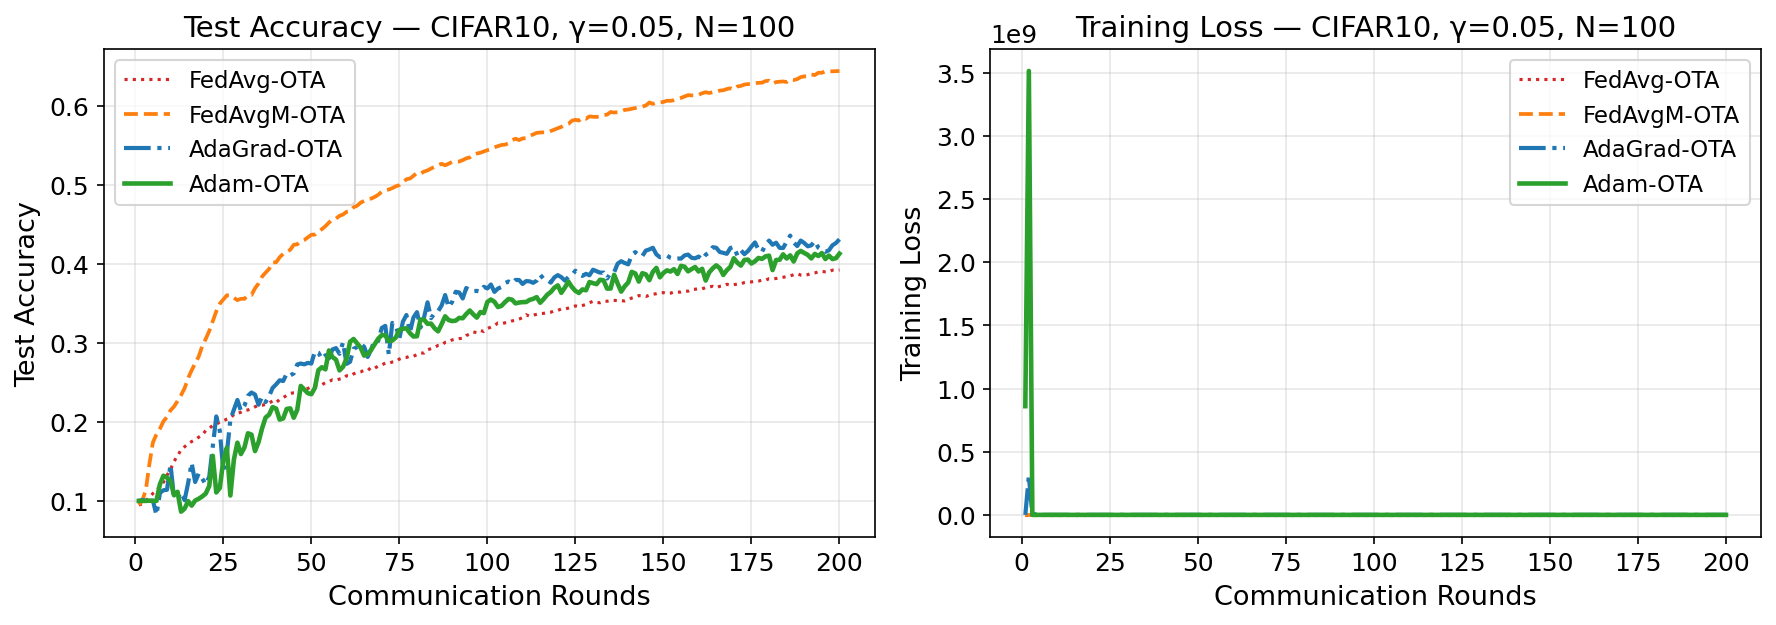
\includegraphics[width=0.95\textwidth]{../results/figures/cifar10_resnet18_alpha2.0_N100_curves.png}
    \caption{CIFAR-10 comparison curves for FedAvg-OTA, FedAvgM-OTA, AdaGrad-OTA, and Adam-OTA.}
    \label{fig:cifar-curves}
\end{figure}

The single-run outputs provide an additional sanity check, but they are not a
controlled four-method comparison because their hyperparameters differ from
Table \ref{tab:config-main}. The single CIFAR-10 Adam-OTA run uses batch size
128 and server learning rate 0.01, reaching 61.51\% final accuracy. The
single MNIST AdaGrad-OTA run uses an IID client split and reaches 97.57\%
final accuracy. These runs confirm that the implemented optimizers can train
successfully, but the main conclusions should be drawn from the controlled
comparison tables above.

\section{Alpha-Stable Tail-Index Ablation}
The revised core experiment varies the alpha-stable tail index instead of
only varying the AWGN scale. The endpoint $\alpha=2$ is Gaussian AWGN, while
smaller values of $\alpha$ produce heavier-tailed impulsive interference.
This is the setting where adaptive normalization is most meaningful: a
server method must handle rare but very large aggregate perturbations.

\IfFileExists{data/generated/alpha_ablation_table.tex}{
    \begin{table}[!htbp]
    \centering
    \small
    \caption{CIFAR-10 alpha-stable tail-index ablation}
    \label{tab:alpha-ablation}
    \begin{tabular}{p{0.26\textwidth}|p{0.48\textwidth}}
        \hline
        Output & Status \\
        \hline
        Alpha ablation & Run the alpha ablation module, then regenerate tables and figures. \\
        \hline
    \end{tabular}
\end{table}

}{
    \begin{table}[!htbp]
        \centering
        \caption{CIFAR-10 alpha-stable tail-index ablation}
        \label{tab:alpha-ablation}
        \begin{tabular}{c|c}
            \hline
            Result file & Status \\
            \hline
            \path{results/heavytail/alpha_ablation_cifar10_resnet18.json}
            & Run \path{./run_all.sh alpha_ablation} and then
            \path{./run_all.sh paper_update} \\
            \hline
        \end{tabular}
    \end{table}
}

\begin{figure}[!htbp]
    \centering
    \IfFileExists{../results/figures/alpha_ablation_cifar10_resnet18_plot.png}{
        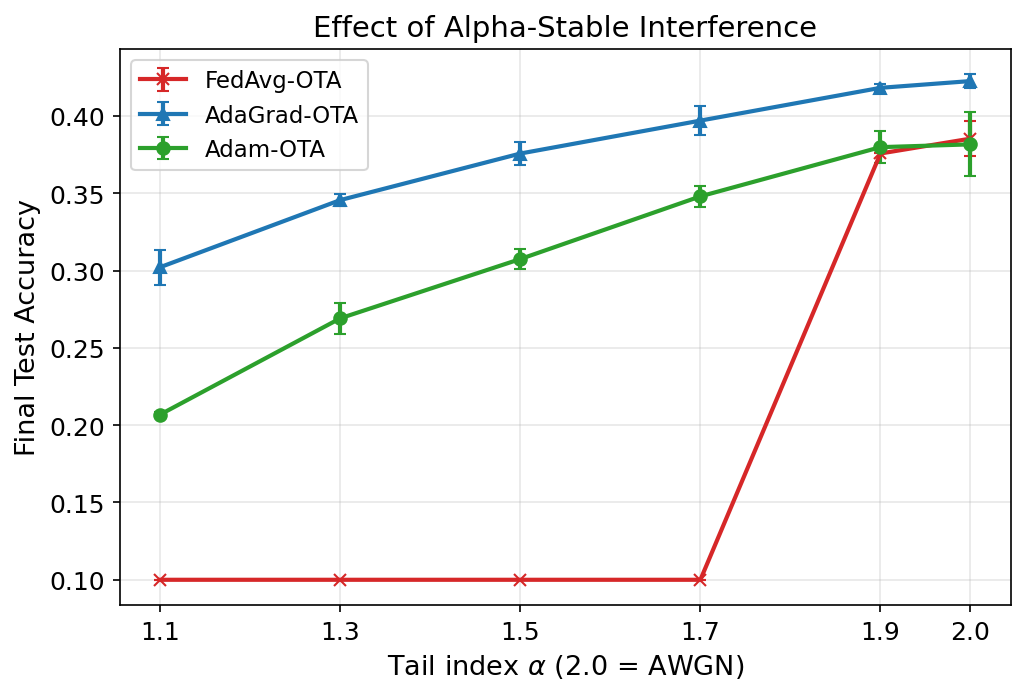
\includegraphics[width=0.9\textwidth]{../results/figures/alpha_ablation_cifar10_resnet18_plot.png}
    }{
        \fbox{\parbox{0.85\textwidth}{\centering
        Alpha-ablation figure is generated by
        \path{./run_all.sh paper_update} after the heavy-tail runs finish.}}
    }
    \caption{CIFAR-10 final accuracy as a function of alpha-stable tail index $\alpha$.}
    \label{fig:alpha-ablation}
\end{figure}

The expected qualitative pattern is that convergence becomes slower and less
stable as $\alpha$ decreases. The adaptive methods should be interpreted
through this heavy-tail curve rather than through an AWGN-only sweep over
$\gamma$.

\section{MAC Robust Pre-Processing}
The second revised experiment compares training with and without Median
Anchored Clipping under a heavy-tailed setting. The default comparison uses
$\alpha=1.3$, $\gamma=0.05$, and clipping factor $k=3$. MAC is not expected
to change the Gaussian endpoint dramatically, but it should reduce the
effect of rare impulsive coordinates when $\alpha<2$.

\IfFileExists{data/generated/mac_compare_table.tex}{
    \begin{table}[!htbp]
    \centering
    \small
    \caption{CIFAR-10 MAC comparison under heavy-tailed interference}
    \label{tab:mac-compare}
    \begin{tabular}{p{0.26\textwidth}|p{0.48\textwidth}}
        \hline
        Output & Status \\
        \hline
        MAC comparison & Run the MAC comparison module, then regenerate tables and figures. \\
        \hline
    \end{tabular}
\end{table}

}{
    \begin{table}[!htbp]
        \centering
        \caption{CIFAR-10 MAC comparison under heavy-tailed interference}
        \label{tab:mac-compare}
        \begin{tabular}{c|c}
            \hline
            Result file & Status \\
            \hline
            \path{results/heavytail/mac_compare_cifar10_resnet18_alpha1.3.json}
            & Run \path{./run_all.sh mac_compare} and then
            \path{./run_all.sh paper_update} \\
            \hline
        \end{tabular}
    \end{table}
}

\begin{figure}[!htbp]
    \centering
    \IfFileExists{../results/figures/mac_compare_cifar10_resnet18_alpha1.3_plot.png}{
        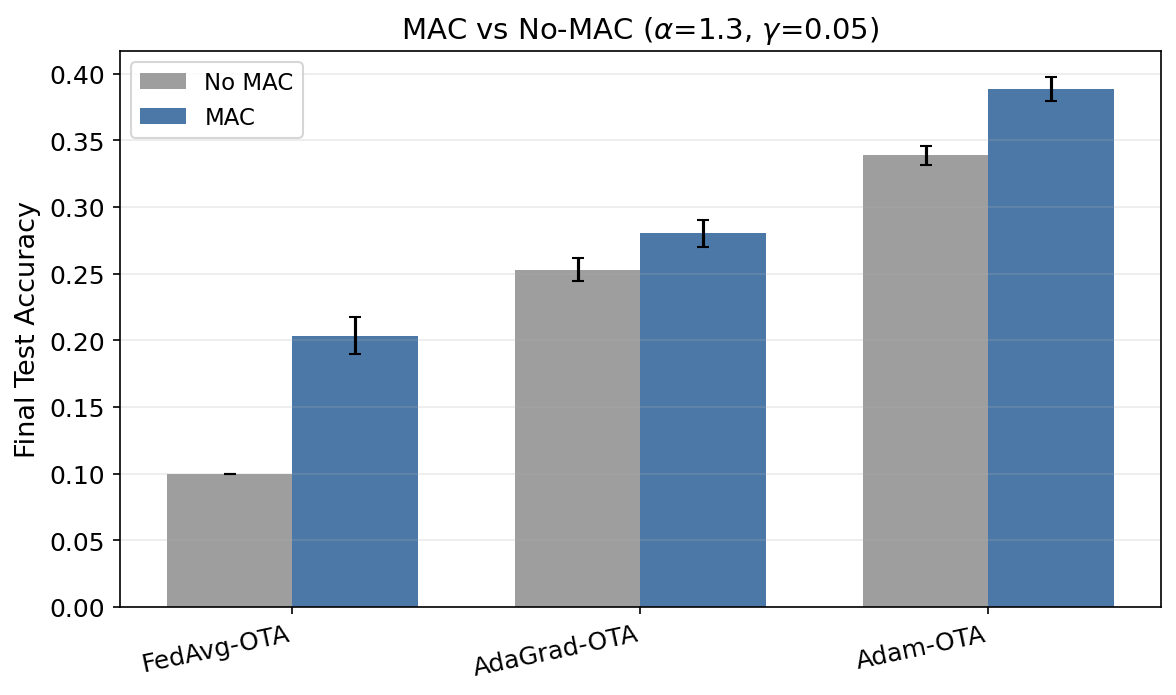
\includegraphics[width=0.9\textwidth]{../results/figures/mac_compare_cifar10_resnet18_alpha1.3_plot.png}
    }{
        \fbox{\parbox{0.85\textwidth}{\centering
        MAC comparison figure is generated by
        \path{./run_all.sh paper_update} after the heavy-tail runs finish.}}
    }
    \caption{CIFAR-10 comparison of no-MAC and MAC under alpha-stable interference.}
    \label{fig:mac-compare}
\end{figure}

\section{Client-Count Ablation}
Table \ref{tab:client-ablation} reports the Adam-OTA client-count
ablation on CIFAR-10. With the same 100-round budget, increasing the number of
clients improves final accuracy from 10.26\% at 5 clients to 21.72\% at 100
clients. This trend is consistent with OTA aggregation: averaging more client
updates can make the aggregate direction more informative, even though the
data remain non-IID and the channel still injects noise.

\begin{table}[!htbp]
    \centering
    \caption{CIFAR-10 client-count ablation with Adam-OTA}
    \label{tab:client-ablation}
    \begin{tabular}{c|c|c|c}
        \hline
        Clients $N$ & Final loss & Final accuracy & Best accuracy \\
        \hline
        5 & 2.3121 & 10.26\% & 10.36\% \\
        10 & 2.2288 & 16.92\% & 16.96\% \\
        20 & 2.1249 & 19.99\% & 19.99\% \\
        50 & 2.1171 & 20.36\% & 20.36\% \\
        100 & 2.0880 & 21.72\% & 21.72\% \\
        \hline
    \end{tabular}
\end{table}

\begin{figure}[!htbp]
    \centering
    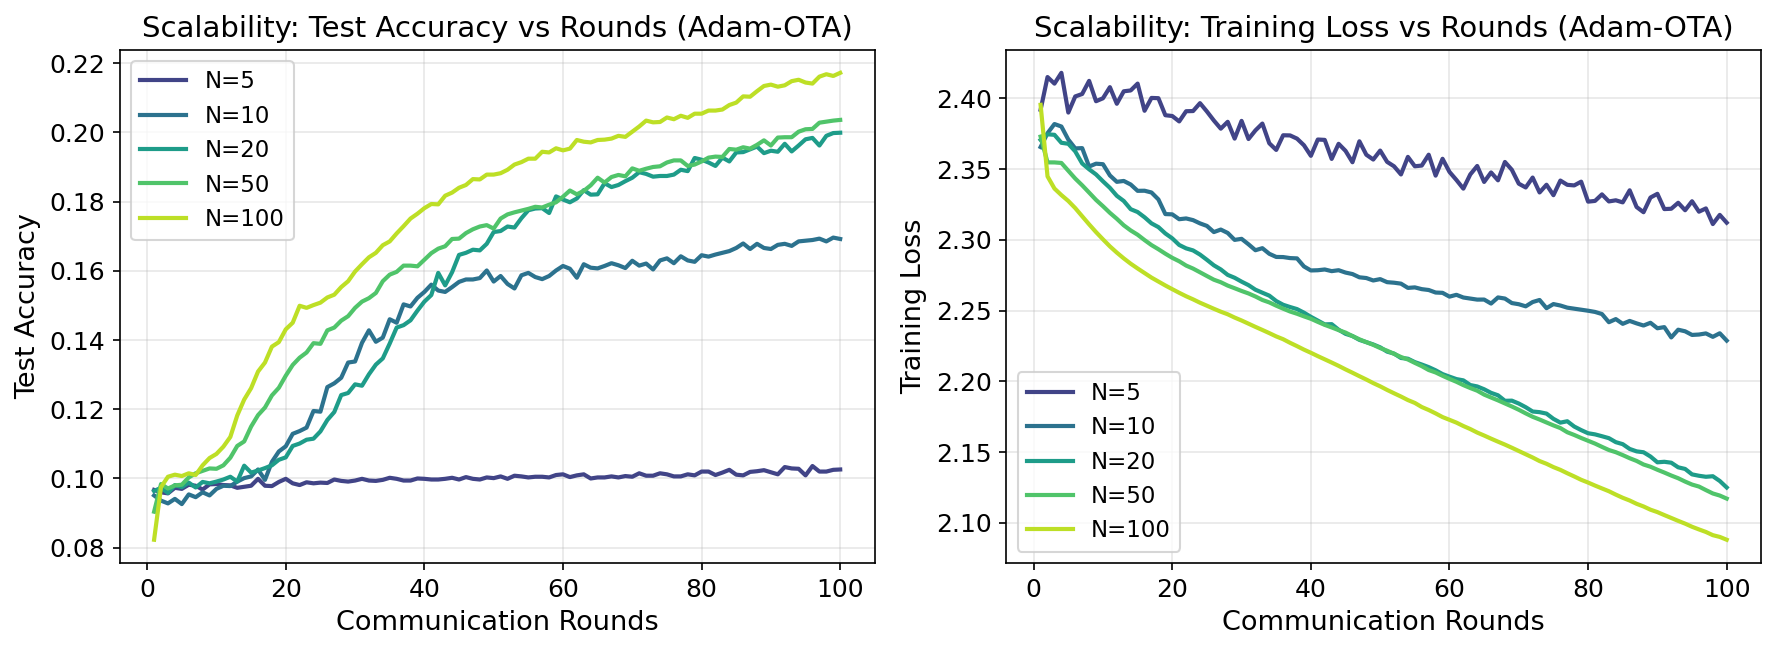
\includegraphics[width=0.95\textwidth]{../results/figures/ablation_clients_cifar10_resnet18_plot.png}
    \caption{CIFAR-10 client-count learning curves for Adam-OTA.}
    \label{fig:client-ablation}
\end{figure}

\section{Discussion}
The experiments should be interpreted in two layers. The existing AWGN
comparison remains a useful endpoint sanity check: it shows that the
implementation trains successfully and that FedAvgM-OTA is a strong CIFAR-10
baseline. The revised alpha-stable ablation is the central evidence for the
project claim, because it tests the heavy-tailed channel condition that
motivates adaptive OTA-FL in the first place.

The project conclusion should therefore be phrased carefully. The results do
not prove that Adam-OTA universally dominates all baselines. Instead, the
claim is that fractional second-moment adaptive updates and robust
pre-processing provide practical mechanisms for improving OTA-FL stability
when the aggregate update is corrupted by alpha-stable impulsive noise. If
adaptive methods underperform FedAvgM-OTA in some CIFAR-10 settings, that is
not a contradiction; it indicates that aggressive normalization can compress
useful signal as well as channel noise.
